\documentclass[two_sides]{my_article}

\usepackage{minted}

\hypersetup{
       backref=false,
       pagebackref=false,
       hyperindex=false,
       colorlinks=false,
       breaklinks=true,
       urlcolor= black,
       linkcolor= black,
       bookmarks=false,
       bookmarksopen=false,
       pdfborder={0 0 0}
}

\lstset{aboveskip=20pt,belowskip=5pt, language=bash, keywordstyle=\color{black}}

\usepackage{pdfpages}

\title{Student and staff IT introduction}
\subtitle{A very brief introduction to UNIX}
\author{Pierre-Yves Dupont - p.y.dupont@massey.ac.nz - ssiti2013@gmail.com}
\date{}

\usepackage{upquote}
\begin{document}
\maketitle

\section{Introduction}
UNIX is an operating system which was first developed in the 1960s, and has been under constant development ever since. By operating system, we mean the suite of programs which make the computer work. It is a stable, multi-user, multi-tasking system for servers, desktops and laptops.
\paragraph{}
There are many different versions of UNIX, although they share common similarities. The most popular varieties of UNIX are Sun Solaris, GNU/Linux, and MacOS X. There are several distributions of Linux: Ubuntu, Debian, Fedora,\dots
All UNIX commands should have the same behavior on all UNIX machines.

\section{The Shell}
The shell is a command line interpreter (CLI). It interprets the commands the types and displays the results. The commands are themselves programs.
The shell allows filename and command name completion using TAB key.
The shell keeps a list of the commands you have typed in. This list is given by the command \emph{history}.

\section{Simple commands}

\subsection{Directory Structure}

All the files are grouped together in the directory structure. The file-system is arranged in a hierarchical structure, like a tree. The top of the hierarchy is traditionally called root (written as a slash / ).

\subsubsection{ls (list)}
When you first login, your current working directory is your home directory. Your home directory has the same name as your user-name, and it is where your personal files and subdirectories are saved.
To find out what is in your home directory, type

\begin{lstlisting}[frame=lines, numbers=none]
ls
\end{lstlisting}

The \emph{ls} command ( lowercase L and lowercase S ) lists the contents of your current working directory.
By default, this command doesn't display hidden files and directories. Files and directories having a name starting by a dot (.) are considered as hidden files on UNIX systems. Hidden files and usually contain important program configuration information. They are hidden because you should not change them unless you are very familiar with UNIX!

To list all files in your home directory including those whose names begin with a dot, type

\begin{lstlisting}[frame=lines, numbers=none]
ls -a
\end{lstlisting}

\emph{ls} is an example of a command which can take options: \emph{-a} is an example of an option. The options change the behaviour of the command. To access to the documentation of most of UNIX commands type

\begin{lstlisting}[frame=lines, numbers=none]
man ls
\end{lstlisting}

This command displays the manual of \emph{ls}.
\paragraph{}
\emph{Remark}: The current directory is represented by one dot (.), the parent directory by two dots (..) and your home directory by a tilde (~).

\subsubsection{mkdir (make directory)}

We will now make a subdirectory in your home directory to hold the files you will be creating and using in the course of this tutorial. To make a subdirectory called \emph{ssiti} in your current working directory type

\begin{lstlisting}[frame=lines, numbers=none]
mkdir ssiti
\end{lstlisting}

\subsubsection{cd (change directory)}

The command \emph{cd directory means} change the current working directory to 'directory'. The current working directory may be thought of as the directory you are in, i.e. your current position in the file-system tree.

To change to the directory you have just made, type
\begin{lstlisting}[frame=lines, numbers=none]
cd ssiti
\end{lstlisting}

To go in the parent directory type

\begin{lstlisting}[frame=lines, numbers=none]
cd ..
\end{lstlisting}

To go to the root of the system, type

\begin{lstlisting}[frame=lines, numbers=none]
cd /
\end{lstlisting}

To go back to your home directory, type

\begin{lstlisting}[frame=lines, numbers=none]
cd
\end{lstlisting}

The command \emph{cd} without any argument returns you to your home directory.

To know where you are in the directories structure, type

\begin{lstlisting}[frame=lines, numbers=none]
pwd
\end{lstlisting}

The command \emph{pwd} displays the \emph{p}ath to the \emph{w}orking \emph{d}irectory.

\subsection{Play with files and directories}

\subsubsection{Create, copy, rename and move}

To create and empty file, type

\begin{lstlisting}[frame=lines, numbers=none]
touch my_new_file
\end{lstlisting}

\emph{Remark}: it's better to avoid to use spaces in file or directory names. You can replace them by underscores (\_)

\paragraph{}
To copy a file, type 

\begin{lstlisting}[frame=lines, numbers=none]
cp file1 file2
\end{lstlisting}

This command  makes a copy of file1 in the current working directory and calls it file2.

To copy a directory, type 

\begin{lstlisting}[frame=lines, numbers=none]
cp -r dir1 dir2
\end{lstlisting}

To move a file, type 

\begin{lstlisting}[frame=lines, numbers=none]
mv file1 file2
\end{lstlisting}

The syntax is really close to \emph{cp} but this has the effect of moving rather than copying the file, so you end up with only one file rather than two.

It can also be used to \emph{rename} a file, by moving the file to the same directory, but giving it a different name.

\paragraph{}
To remove a file, type

\begin{lstlisting}[frame=lines, numbers=none]
rm file1
\end{lstlisting}

To remove a directory, you can use

\begin{lstlisting}[frame=lines, numbers=none]
rm -r directory
\end{lstlisting}

With the \emph{-r} option \emph{rm} will remove all files in the directory then the directory. Be careful!!

\subsubsection{Display text files}

To look at the contents of a file, you can use

\begin{lstlisting}[frame=lines, numbers=none]
cat file1.txt
\end{lstlisting}

This command shows the entire file. That’s fine for an 8 KB file, but you wouldn’t want
to use this command on a 5 GB file!
\paragraph{}
To  look at the file in pieces, use

\begin{lstlisting}[frame=lines, numbers=none]
less file1.txt
\end{lstlisting}

In the \emph{less} program, you can move using the arrows. Use 'q' to quit. Some useful options for \emph{less} command:
\begin{itemize}
\item \emph{-S}: Causes lines longer than the screen width to be chopped rather than folded
\item \emph{-N}: Causes a line number to be displayed at the beginning of each line in the display
\item hit \emph{slash} in less environment to search a word (\emph{n} and \emph{N} keys to find next and previous occurrence)
\item enter a line number in less environment to go to the given line
\end{itemize}
\paragraph{}
If the file is really big, it may be better to use the \emph{head} and \emph{tail} commands.

\begin{lstlisting}[frame=lines, numbers=none]
head -n 8 file1.txt
tail -n 8 file1.txt
\end{lstlisting}

\emph{head -n 8} displays the 8 first lines of the file. \emph{tail -n 8} displays the 8 last lines.
\paragraph{}
It's possible to combine the two commands

\begin{lstlisting}[frame=lines, numbers=none]
head -n 50 test_fasta_file.fna | tail -n 10
\end{lstlisting}

Using this command, you will display the lines 40 to 50 of your file. The pipe (\textbar) character is used to redirect the output of the first command (\emph{head}) to the second (\emph{tail}).

\subsubsection{More useful commands on files}

Counting the number of lines in a file:

\begin{lstlisting}[frame=lines, numbers=none]
wc -l file1.txt
\end{lstlisting}

\emph{wc} command can be also used to count the number of characters in a file:

\begin{lstlisting}[frame=lines, numbers=none]
wc -m file1.txt
\end{lstlisting}

and also to count the number words:

\begin{lstlisting}[frame=lines, numbers=none]
wc -w file1.txt
\end{lstlisting}

To find the lines containing a pattern:

\begin{lstlisting}[frame=lines, numbers=none]
grep '>' file1.txt
\end{lstlisting}

This command will return all the lines of the file containing the pattern '\textgreater'. By default, the search is case sensitive, to ignore the case, use \emph{-i} option.

To count the number of line containing a pattern:

\begin{lstlisting}[frame=lines, numbers=none]
grep -c '>' file1.txt
\end{lstlisting}

Here, the command returns the number of line containing the character '\textgreater'. To count the number of '\textgreater' in the file, you can use:

\begin{lstlisting}[frame=lines, numbers=none]
grep -o '>' file1.txt | wc -l
\end{lstlisting}

If you are interested in having only the number of lines starting by '\textgreater', use the following command:

\begin{lstlisting}[frame=lines, numbers=none]
grep -P -c  '^>' file1.txt
\end{lstlisting}

The sign '\textasciicircum' means 'beginning of the line'. If you want to find the number of lines ending by a dot (.) use the following command:

\begin{lstlisting}[frame=lines, numbers=none]
grep -P -c '\.$' file1.txt
\end{lstlisting}
%$
The sign '\$' means 'end of the line'. The dot is a special character for grep meaning 'any alphanumeric character', so if you are looking for a real dot, you have to \emph{escape} it using the backslash (\textbackslash) sign.

\subsubsection{Output Redirection}

On UNIX it's possible to redirect the output of a command to a file. To do that we use \textgreater\space sign.

\begin{lstlisting}[frame=lines, numbers=none]
ls > myfile.txt
\end{lstlisting}

This command writes the results of the \emph{ls} command in the \emph{myfile.txt}. If the file doesn't exists, it will be created, if it exists it will be erased and recreated. It's also possible to append a the end of a file:

\begin{lstlisting}[frame=lines, numbers=none]
ls >> myfile.txt
\end{lstlisting}

\subsubsection{CSV and Tab delimited files}

UNIX is really efficient to work on files containing columns of data delimited by a separator (tabulation, comma\dots). For example, it's possible to sort a large file given a column in some seconds.

\begin{lstlisting}[frame=lines]
sort -k 2 -n file1.txt
sort -k 2 -n -r file1.txt
\end{lstlisting}

The first line correspond to a sort of a space delimited file (default format for \emph{sort} command) on the second column using a numeric sort. The line two correspond to a reverse sort of the file. To use \emph{sort} command on CSV files (delimited by a comma), you must specify a delimiter:

\begin{lstlisting}[frame=lines, numbers=none]
sort -k 2 -n -t$',' file2.csv
\end{lstlisting}
%$

It is also possible to sort on more than one column:
\begin{lstlisting}[frame=lines, numbers=none]
sort -k1,1n -k2,2 -t$',' file2.csv
\end{lstlisting}
%$

Here \emph{file2.csv} will be sorted first on the first column (\emph{-k1,1n}) using a numeric sort (\emph{n}) then on the second column (\emph{-k2,2}).

Sometime it can be useful to make a sort on a file ignoring the first line (header line). To do that you must combine three commands:

\begin{lstlisting}[frame=lines, numbers=none]
(head -1 file.csv ; tail -n +2 file.csv | sort -t$',' -k1,1 -k2,2n) > file2.csv
\end{lstlisting}
%$

\emph{tail -n +2 file.csv} displays all the lines of the file ignoring the first line. The result of that command is used in the sort (\emph{ sort -t\$',' -k1,1 -k2,2n}). To print the header line in the result file (\emph{file2.csv}) you have to execute ``\emph{head -1 file.csv}'' command which displays only the first row of the file. 

\paragraph{}
It is also easy to extract columns from a file:

\begin{lstlisting}[frame=lines, numbers=none]
cut -f2-4,6 -d$'\t' file1.txt
\end{lstlisting}
%$

This command extracts the columns 2 to 4 (2-4) and 6 (,6) in a tab delimited file.

It is also possible to display huge delimited files (impossible to display in MS-Excel or equivalent software) using the \emph{column} command.

\begin{lstlisting}[frame=lines, numbers=none]
column -s $'\t' -t -n < file.txt
\end{lstlisting}
%$

In this command, the option \emph{-s} allows to set a delimiter character, the option \emph{-t} ask to the command to determine automatically how to display the result and \emph{-n} prevent the command to merge the consecutive delimiters.

It is also possible to find unique sequential entries in a file using;

\begin{lstlisting}[frame=lines, numbers=none]
uniq file.txt
\end{lstlisting}

You can use the option \emph{-c} to only count the number of unique sequential lines in a file.

If you want to change the delimiter of a file you can entrer:

\begin{lstlisting}[frame=lines, numbers=none]
sed -i 's/;/\t/g' file.txt
\end{lstlisting}

This command will substitute (\emph{s}) all (\emph{g} global) ';' by a tabulation '\textbackslash t' in the given file. It replace the file, so be sure to make a copy first. It is also possible to write:

\begin{lstlisting}[frame=lines, numbers=none]
tr ';' '\t' < file.txt
\end{lstlisting}

\paragraph{}
It is also possible to join two files. First ``horizontally'':

\begin{lstlisting}[frame=lines, numbers=none, language=bash]
paste -d$'\t' test_file1.txt test_file2.txt
\end{lstlisting}
%$

This command will produce a file containing the columns from the first file then the columns from the second. Take care of the order first.

\begin{lstlisting}[frame=lines, numbers=none, language=bash]
join -j1 -t$'\t' test_file1.txt test_file2.txt
\end{lstlisting}
%$

This command will join the two files using the first column as reference (\emph{-j1}). If two values are identical in the reference column, \emph{join} will concatenate the values from the two files. The rows from one file which are not in the other will be ignored.

Finally it's also possible to join two files 'vertically' using the command cat:

\begin{lstlisting}[frame=lines, numbers=none, language=bash]
cat test_file1.txt test_file2.txt
\end{lstlisting}

\section{Text file edition}

\subsection{Microsoft Word}

Microsoft Word (and its free versions like OpenOffice and LibreOffice) are not considered as text editors but as word processors. A word processor is a computer application used for the production (including composition, editing, formatting and possibly printing) of any sort of printable material. These software append hidden characters to the text. These characters may be copied when you copy and paste the text! 
\paragraph{}
The size of pure text file containing only the sentence ``Hello World'' is 12bytes. The size of a \emph{docx} document containing exactly the same sentence is 3.4KB (283 times more than the text file!).
\paragraph{}
If you want to work on pure text files, you must use simple text editors.
Text editors can be Smultron or Text Wrangler on MacOS; Wordpad or Notepad++ on MS Windows and Vi, emacs or nano on UNIX. 

\paragraph{}
\emph{Remark}. Emacs, Vi and nano are available also on MS Windows and MacOS.

\subsection{Nano}
The easiest text editor on UNIX is nano. This editor is inside the shell, there is no graphical interface, so it is possible to use even if you don't have access to a graphical session (for example on all computation servers). To open a file using nano, type:

\begin{lstlisting}[frame=lines, numbers=none, language=bash]
nano file.txt
\end{lstlisting}

All available commands are displayed at the bottom of the screen. '\emph{\textasciicircum G}' means \emph{Control+g}. This command display the help of nano. To save, use '\emph{\textasciicircum O}', to exit use '\emph{\textasciicircum X}'. 

\paragraph{}
\emph{Remark}
The Undo/Redo function are, most of the time, not available. On some UNIX and Linux distributions, it is possible to give a \emph{-u} option allowing to have an access to theses functions using M-U (understand Meta-U aka ESC-U) to undo and M-E to redo.

\section{Linux Cheat Sheet}
For a good UNIX cheat sheet, you can go to \url{http://www.cheatography.com/davechild/cheat-sheets/linux-command-line/}
For a very complete list of commands, you can have a look to the UNIX Toolbox reference website: \url{http://cb.vu/unixtoolbox.pdf}

\paragraph{}
A simple cheat sheet on next page
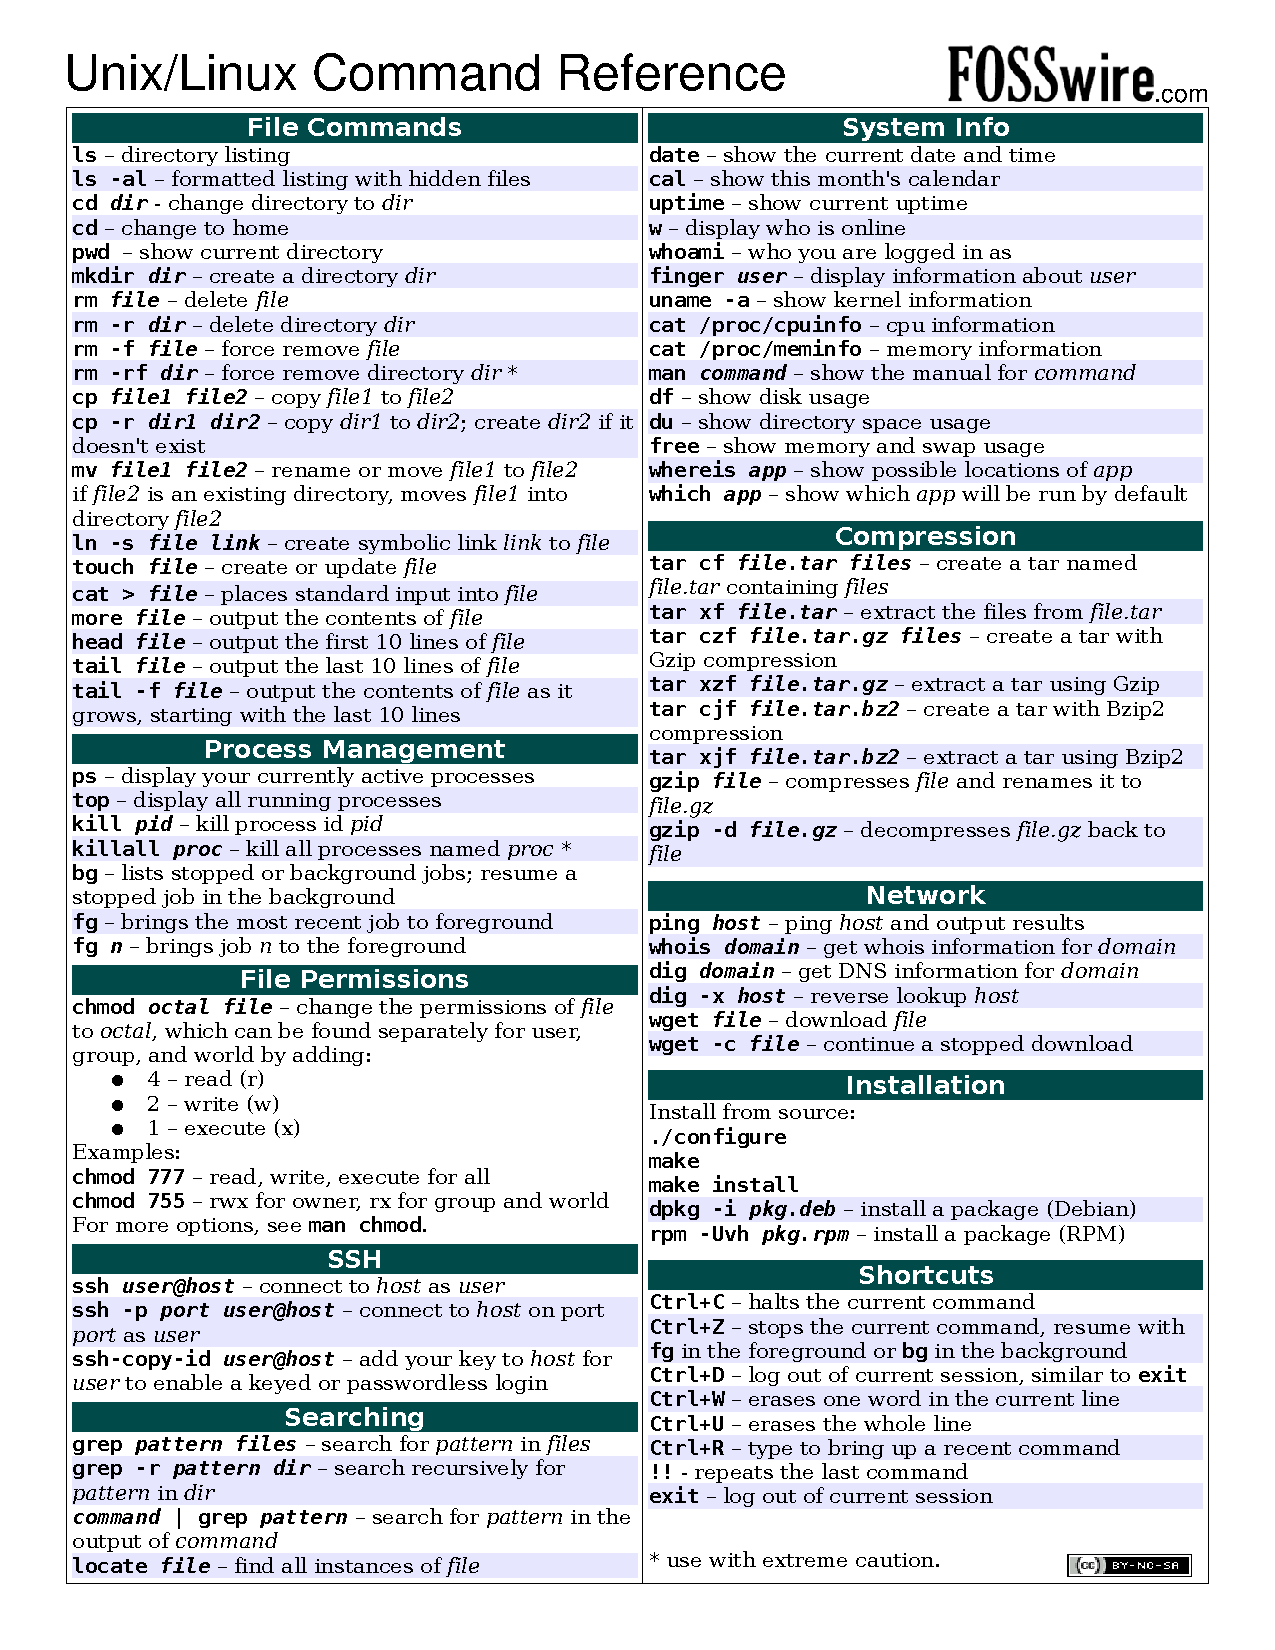
\includepdf{fwunixref.pdf}

\end{document}
%%% Local Variables: 
%%% mode: latex
%%% TeX-master: t
%%% End: 
